\documentclass[11pt]{article}
\usepackage{fullpage,amsmath,mathtools, algorithm2e, forest}
\usepackage[mathletters]{ucs}
\usepackage{hyperref}
\usepackage[utf8x]{inputenc}
\usepackage{graphicx}
\usepackage{listings}
\usepackage{courier}

\lstset{basicstyle=\footnotesize\ttfamily,breaklines=true}
\lstset{frame=single}

\graphicspath{ {./images/} }
\title{COMP 4601 - Assignment 2}
\author{Student Name: Brian Ferch\\
\text{Student Number: 100962115}\\\\ 
Student Name: Jules Kuehn\\
\text{Student Number: 100661464}}
\date{Winter 2019}
\begin{document}
\maketitle


\section{Generating user profiles from reviews}

A wealth of metadata was contained within the /reviews/ HTML files. This included:

\begin{itemize}
    \item Movie ID (ex. B0000D0XZ4)
    \item User ID (ex. A1A69DJ2KPU4CH)
    \item User profile name (ex. James Ferguson)
    \item Rating of movie (ex. 5.0)
    \item Review helpfulness (ex. 64/74)
    \item Review time (ex. 1287273600)
\end{itemize}

We scraped all of this data except the review times, although this data has value as well (see "Future work" below). For the purposes of this assignment, the simplification / assumption is that users have static preferences over time.\newline

While it is certainly possible to do sentiment analysis on the individual reviews (as we have done for the in-class assignment), we felt that given these "true" user ratings, it made more sense to make use of this explicit data than any extracted sentiment. So, the reviews data was processed into the following format:

\begin{itemize}
    \item A "ratings table" where each row label is a User ID, and each column label is a Movie ID. The data contained in this table is the rating of the movie. The rating scale is from 1 to 5, but we stored the values as between 0 and 1, with a value of -1 for a movie not reviewed by this user. The formula for converting star ratings to the range 0 to 1 is $rFloat = \frac{(rStar-1)}{4}$.
    \item A "helpfulness table" corresponding with the same dimensions and labels as above, but storing the helpfulness of each review (parsed to a float)
    \item A map from User ID to User profile name
\end{itemize}

Given this information, some useful characterizations can be made on each user. Included in each of our user profiles is that user's:

\begin{itemize}
    \item Average star rating
    \item Average helpfulness (as rated by other users)
    \item Community affiliation
    \item Position in relation to other users in 2d space
\end{itemize}
% The process by which the community affiliation and 2d representation were obtained is described below.


\section{Clustering users into communities}

The ratings table is large: 1252 rows (users) x 1079 columns (movies). It is also very sparse (93.9\% empty). We first reduced this to a dense, low-dimensional representation by the following process:

\begin{enumerate}
    \item Calculate average ratings for each movie, each user, and the overall average
    \item Fill the missing ratings with the movie's average rating, adjusted to the user's average rating: $rFill = movieAvg + userAvg - overallAvg$
    \item Normalize the matrix to adjust for user average ratings in general.
    \item Determine an appropriate number of dimensions $k$ for truncation.
\end{enumerate}

Reconstructing the original matrix from the 2-dimensional truncated SVD yields an error of 29.2\% without filling or normalization. After filling and normalization though, the error is reduced to 23.7\%. Truncating at 200 dimensions, this error drops to 9.3\%. However, this has little effect on the clustering of users. We can see below that the user clusters determined from the 200-dimensional representation are very similar to the 2-dimensional representation, and that the vast majority of the variance occurs in a single dimension.

\begin{figure}[h!]
    \centering
    \begin{minipage}{0.45\textwidth}
        \centering
        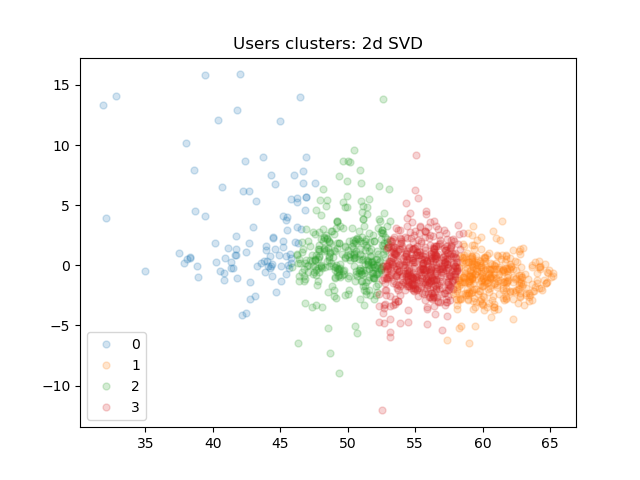
\includegraphics[width=0.9\textwidth]{user_clusters_2d} % first figure itself
        \caption{Kmeans clustering on users in 2d}
    \end{minipage}\hfill
    \begin{minipage}{0.45\textwidth}
        \centering
        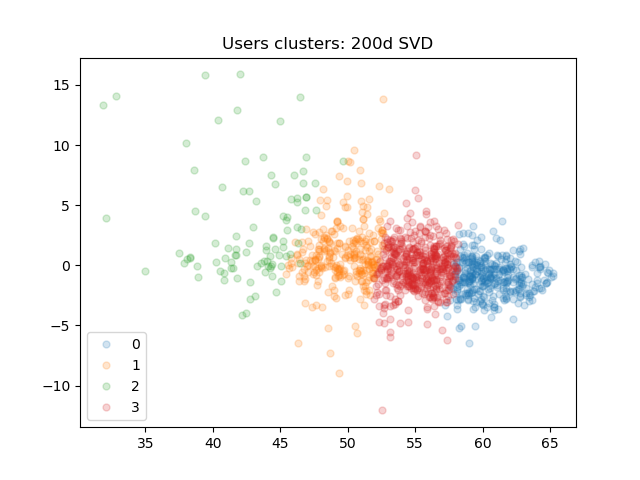
\includegraphics[width=0.9\textwidth]{user_clusters_200d} % second figure itself
        \caption{Very similar results in 200d}
    \end{minipage}
\end{figure}

Given these results, we used a 2-dimensional representation for users. We determined the best number of clusters to be $m = 4$ based on elbow finding in both 2d and 200d. The process ultimately generated two useful mappings: User ID to 2D representation, and User ID to community number.

\begin{figure}[h!]
    \centering
    \begin{minipage}{0.45\textwidth}
        \centering
        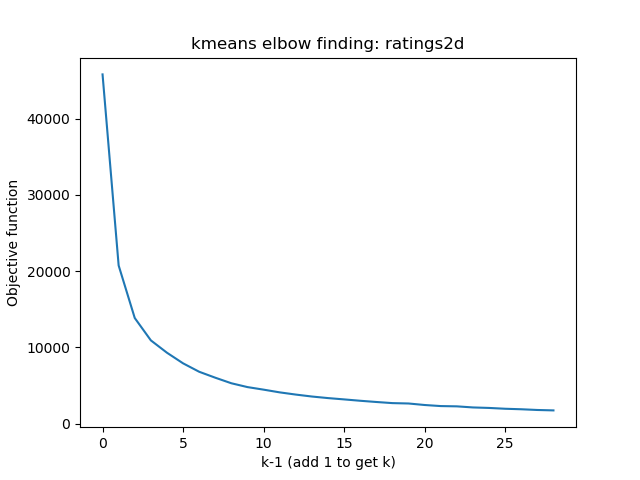
\includegraphics[width=0.9\textwidth]{kmeans_elbow_2d} % first figure itself
        \caption{Suggests 4 clusters of users}
    \end{minipage}\hfill
    \begin{minipage}{0.45\textwidth}
        \centering
        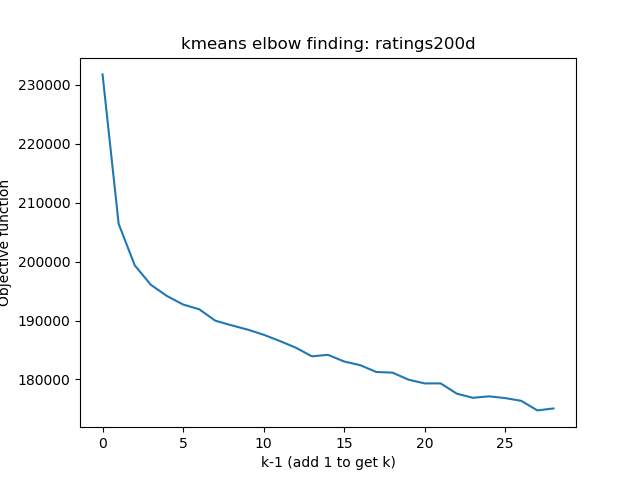
\includegraphics[width=0.9\textwidth]{kmeans_elbow_200d} % second figure itself
        \caption{Similar results in 200d}
    \end{minipage}
\end{figure}


% \lstinputlisting{results/results.txt}

% \begin{figure}[h!]
%     \centering
%      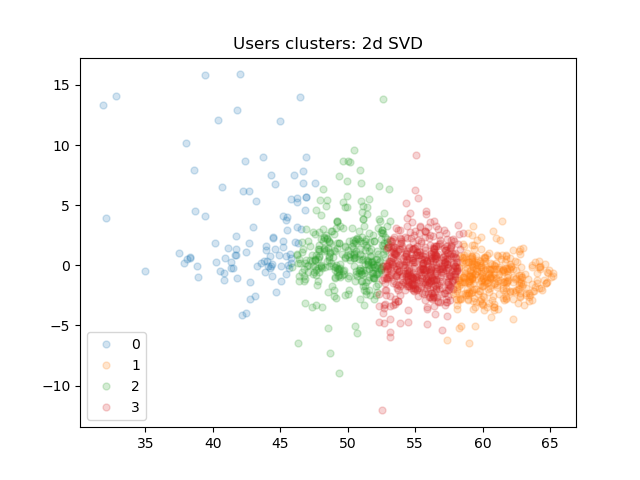
\includegraphics[width=0.5\textwidth]{user_clusters_2d}
%         \caption{Percentage of Recognition Errors}
% \end{figure}

\section{Topic analysis on movies according to page text}

We could create some approximation of genre for each movie by extracting topics from the pages with the following process:

\begin{enumerate}
    \item Calculate LDA topics on review pages (since each page corresponds to one movie).
    \item For each page, we take the topic with the maximum distribution value and call this the movie's topic.
\end{enumerate}

Tinkering with the parameters of LDA iteratively led us to topics that progressively came closer to mimicking genre.

We strived to keep our distributions fairly biased to one topic since only the max was considered. Four topics
ended up being the sweet spot that gave us this behavior.

Stop words were added at each iteration as they appeared in the generated topics. In addition to conventional stop words,
topic words that were too general and not indicative of genre like "movie" or "film" were added.

\begin{figure}[h!]
    \centering
    \begin{minipage}{0.45\textwidth}
        \centering
        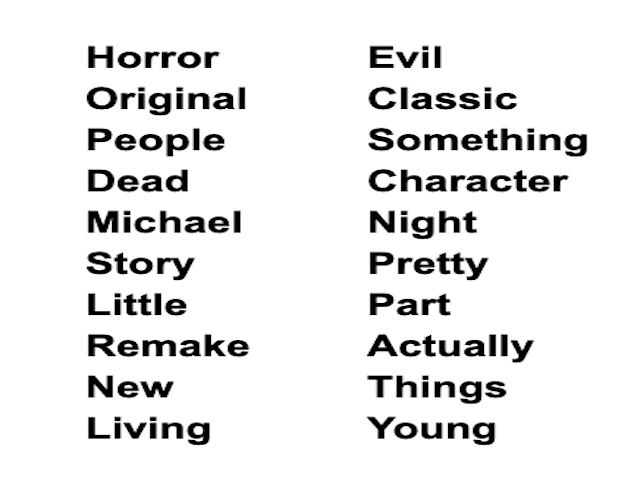
\includegraphics[width=0.9\textwidth]{horrortopic}
        \caption{Example "horror" topic}
    \end{minipage}\hfill
    \begin{minipage}{0.45\textwidth}
        \centering
        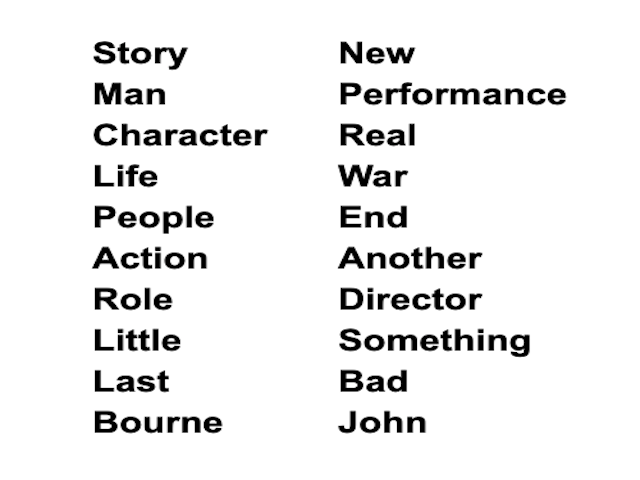
\includegraphics[width=0.9\textwidth]{waractiontopic} % second figure itself
        \caption{Example "war action" topic}
    \end{minipage}
\end{figure}


\section{Generating and retrieving contextual advertisements}

Having now generated $m = 4$ user communities and $n = 4$ movie topic categorizations, we create $m * n = 16$ advertising categories, one for each combination of \{community, topic\}.\newline

Advertising for each community is comprised of "recommended movies" for that community. These movies are determined by:

\begin{itemize}
    \item Creating a community ratings matrix where the ratings are the averages of all ratings from users in that community for a particular movie (or -1 if no users in this community rated the movie)
    \item Finding the movies for each community which are rated better (by that community) than the community average
\end{itemize}

An advertisement is generated for a specific \{user/page\} by:

\begin{itemize}
    \item Retrieving all recommended movies for the user's community
    \item Shuffling this list so as to provide sampling from the long tail, rather than just the best rated movie
    \item Taking the first movie from the shuffled list that matches the topic of the current page (or a random recommended movie if the community has not recommended any for this topic)
    \item Generating some HTML which includes the recommended movie's star rating and a link to reviews
\end{itemize}


\section{SUGGEST algorithm}

...


\section{Improvements}

For this assignment we made the assumption that users have static preferences over time. In reality, this is not a good model for profiling users. Since the metadata of the reviews include timestamps, we could profile the users based only on recent behaviour - or even predict the trajectory of user preferences. Taking a sliding window of user behaviour over time would yield a different (2d) representation for the same user at different time stamps. From this, we can use regression to predict the 2d representation of the user at some point in the future, and use this representation for generating advertising.\newline

Upon inspection of the user ratings, we found that they were strictly integers from the set \{1, 2, 3, 4, 5\}. Instead of filling the sparse matrix with item averages (which, in such a sparse matrix, can "smear" the useful information towards the mean) we could use a one-hot encoding on the integer ratings.\newline

Different techniques could be tried for creating lower-dimensional representations of users, including PCA and t-SNE. This could improve clustering.\newline

The helpfulness of a review, or the average helpfulness rating for a user, could be used to give increased weight to high quality reviews.\newline

Improvements can be made to the cleaning and parsing of the HTML. We noticed that there were duplicate reviews in the dataset corresponding to duplicate pages (movies which have the same reviews, but different IDs). These should ultimately be removed from the dataset before processing. The reviews HTML also included the title of each review, which should be included in the text used for LDA topic categorization.\newline.

Experimentation with different stopwords may also lead to better results in the LDA process. The categorization process could be enhanced by creating document vectors for each of the pages (a concatenation of movie reviews, ideally augmented with the review titles). In the same format, we would create document vectors for reviews of movies for which we know the category, and train a neural net on this latter set. Our pages would then be predicted to a known category, which would likely provide a more meaningful categorization than the unsupervised bag-of-words approach we took for the assignment.

\end{document}